%File: formatting-instruction.tex
\documentclass[letterpaper]{article}
\usepackage{aaai}
\usepackage{times}
\usepackage{helvet}
\usepackage{courier}\usepackage{graphicx}
\graphicspath{ {./imgs/} }
\frenchspacing
\setlength{\pdfpagewidth}{8.5in}
\setlength{\pdfpageheight}{11in}
\pdfinfo{
/Title (Insert Your Title Here)
/Author (Put All Your Authors Here, Separated by Commas)}
\setcounter{secnumdepth}{0}  
 \begin{document}
% The file aaai.sty is the style file for AAAI Press 
% proceedings, working notes, and technical reports.
%
\title{GPT3 In the pursuit to easily query\\ Genomic Knowledge}
\author{S. Solomon Darnell\\
UTHSC Department of Genetics, Genomics and Informatics (GGI)\\
71 S. Manassas Street, 4th Floor\\
Memphis, Tennessee 38163\\
e $->$ genetics@uthsc.edu, solo.shelby@proton.me
}
\maketitle
\begin{abstract}
\begin{quote}
The advent of popular and useful large text search and generative artificial intelligence (AI) has led to the automation of many rote tasks and more amazingly multiple creative ones as well.
\end{quote}
\end{abstract}



\noindent Scholars world wide spend exhaustive amounts of time and effort reading, summarizing, converting, memorizing, and mixing knowledge for their own purposes, and to push science forward.
Since the inception of AI its promise has exponentially out-sized its capabilities; however, computing resources strong enough to exploit deep learning in conjunction with continual improvements in the use and management of `big data' have begun to close the gap between `perceived utility' and promise of AI.
`Perceived utility' is how the common person understands AIs use and helpfulness.
There are AI utilities, applications, and algorithms that are used widely for automation, recognition, navigation, semi-autonomous vehicles, mars rover exploration, deep question answering, and now creativity.
The essence of AI is getting computers to perform `intelligent' human tasks.
Pursuit of the same has caused some researchers to thoroughly examine and re-examine their definitions of intelligence.
Many see a humanoid android or automaton that is difficult to differentiate from a human as the pinnacle of AI; because AI as a field has so many areas in which it needs to improve to reach such a technical height, it is defined with many sub-fields.
The major sub-fields of AI include: machine learning, natural language processing, 
\cite{2022Azaria,2023Zhang,2023Foucart,2023DePeau-Wilson}

%\iffalse
\section{What is needed to train a GPT3 level LLM}
\subsection{Training with MosaicML}

To train BioMedLM easily, quickly, and efficiently, we used the MosaicML Cloud for infrastructure and trained the model using MosaicML’s Composer and Streaming Dataset libraries. All model and training code is built off of PyTorch. See the code here!

\subsubsection{MosaicML Cloud}
Using our cloud software stack, we orchestrated training on top of a cluster with 128 NVIDIA A100-40Gb GPUs and 1600 Gb/s networking bandwidth between nodes. 
The physical GPUs were hosted on a leading cloud provider. The total training time for BioMedLM was \~ 6.25 days. 
Using placeholder pricing of \$2/A100/hr, the total cost for this training run on MosaicML Cloud was \~ \$38,000. 

\subsubsection{Composer}
For the optimal LLM training experience, we used Computer with its FSDP integration (FDSP is a PyTorch backend for fully sharded data parallel training). 
The open-source Composer library makes it easy to train large, custom models across hundreds of GPUs without imposing any restrictions on the model code. 
For example, we replaced the HuggingFace GPT2 model attention implementation with FlashAttention (Dao et. al), which improved training throughput by nearly 2x while producing a math-equivalent model. 
Composer had no trouble handling the custom model definition, and training time was cut in half! Having the flexibility to easily add and test modifications greatly improved the training efficiency of BioMedLM, and we expect to make similar improvements in future LLM work.

\subsubsection{Streaming Datasets} 
To manage a training dataset containing over 100GB of text in a cloud-native way, we used MosaicML's new StreamingDataset library.
This library enables users to host arbitrary data (text, images, etc.) as shards in object storage and then stream that data to a training job anywhere in the world. 
StreamingDataset works out of the box with vanilla PyTorch DataLoaders, and is compatible with multiple CPU workers, multi-GPUs, and multi-node training. 

StreamingDataset made it fast, flexible, and cheap for us to manage a custom training dataset. 
There was no need to pre-tokenize the data; we were able to store the samples as raw text in object storage. 
At runtime, we streamed in text samples and tokenized on-the-fly, with no impact on training throughput and no data loader bottlenecks. 
This flexibility and performance enabled us to test different tokenization schemes for BioMedLM without having to regenerate the dataset.

As one last proof point for StreamingDataset, our final training run for BioMedLM did not use compute from AWS, despite the fact that the dataset was stored on AWS S3. 
Instead, we streamed the data from S3 to MosaicML Cloud without impacting training throughput, and without downloading the whole dataset at the start. 
Instead, shards were streamed in as they were needed during the training run and cached after the first epoch. 
This limited the cost of data egress to <\$10 for the whole training run, compared to ~\$38,000 for the compute!

\section{Which model is better for limited datasets?}
\subsection{Is there a sweet spot?}

\section{Building an LLM for research that uses the GeneNetwork Genomics database}

\section{LLM Strengths}
\subsection{Generative AI for Creativity}
\begin{figure}[ht]

\includegraphics[width=8cm]{imgs/African_Woman_Steampunk.eps}
\caption{African Woman in Steampunk Style}
\end{figure}

\begin{figure}[ht]
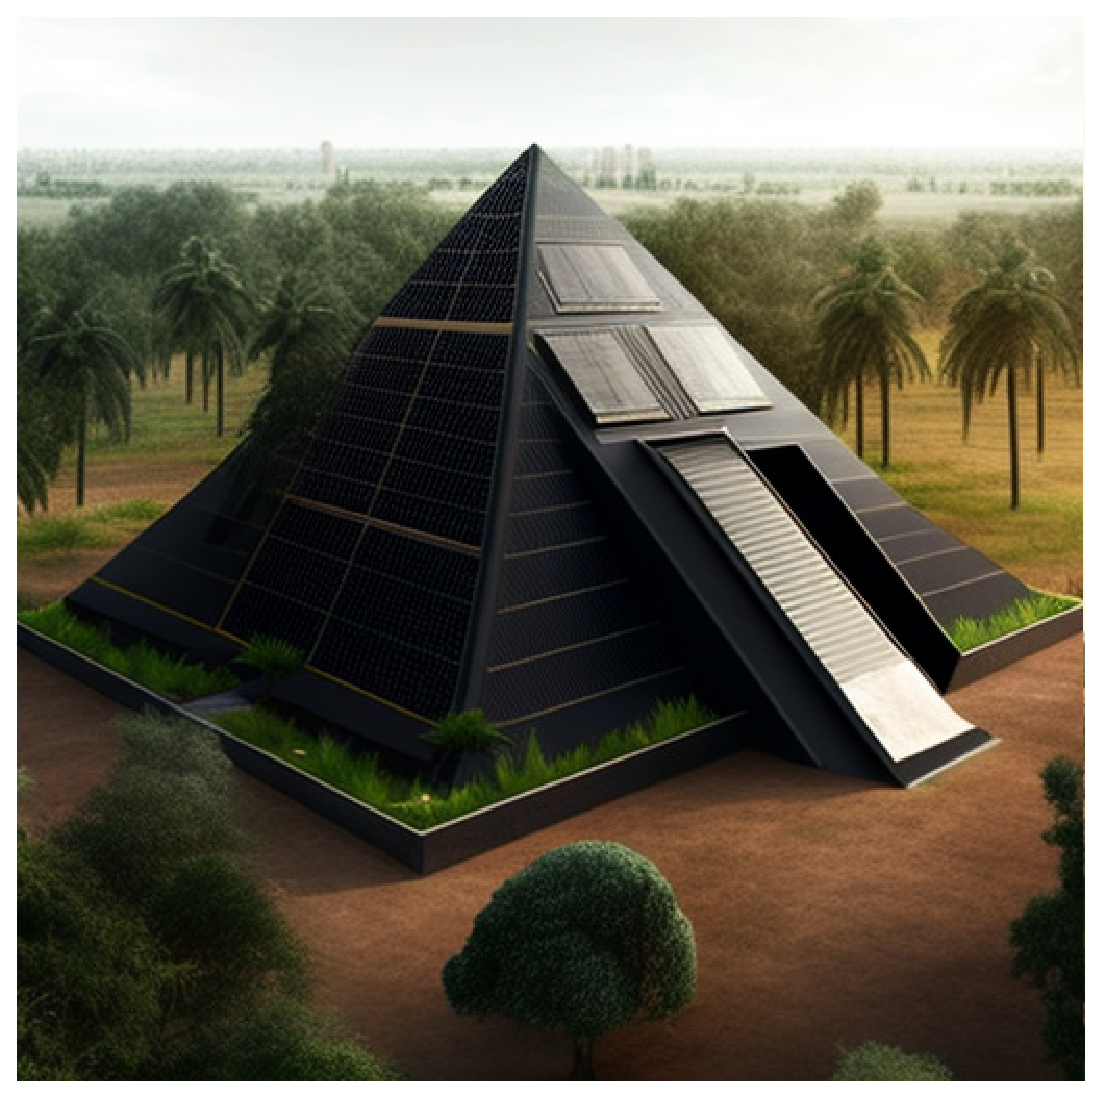
\includegraphics[width=8cm]{imgs/Sudanese_Solar_Pyramid.eps}
\caption{Sudanese Pyramid in a Modern style using Today's solar technology}
\end{figure}

\section{LLM Weaknesses}

\section{Mitigating the weaknesses of an open LLM}

\section{Towards the improvement of a GN.org LLM}
\subsection{What lessons were learned from IBMs 2010 super AI system, Watson?}
\section{Improving LLMs with Causality} % the Conclusion
%\fi

\section{ Acknowledgments}
Many thanks to the Kenyan startup `Fahamu AI' that helped us demo the first version of the GeneNetwork knowledge machine.

%\bigskip
%\noindent Thank you for reading these instructions carefully. We look forward to receiving your electronic files!

\begin{small}
\bibliographystyle{aaai}
\bibliography{refs/scholar,refs/blog}
\end{small}

\end{document}